\subsection{Performance on partial ground truth data}

\jovo{need to discuss preprocessing

fig 1a: include all data in main, in supplement, include current 1a and with errorbars

table of run times

compare with DPMM

check matlab initializes with hierarchical clustering for GMM \& k-means

add waveforms over time in PC space

scatterplot of waveforms of TP, FP, and FN in PC space (either learned from all data or only these waveforms).  let's see whether the distributions look different at all in this space, which should inform us with regard to how well we are doing. perhaps plot ellipsoids (corresponding to level-sets) with means and covariances fit from the data

show waveforms in 3b and 3c in PCA of channel 3 to show that they are overlapping. {\color{green} done}


rotate 3a and 4a panels to be N rows and 1 column, rather than 1 row and N columns

show that we capture waveform adaptation, via showing the $\mu$ moving around in PC space

show 10 waveforms of AR and non-AR means \& errorbars over time 


for overlapping, show in black dashed lines, the "expected" trace (sum of overlapping),
and beside that, show the three time-varying residuals, reporting the sum-squared residuals

then let's plot the two distributions of sum-squared-residuals (one for assuming overlapping, one for only the ground-truth neuron).  depending on how different those two distributions look and what they look like, we can test to demonstrate the differences.


}

\subsection{Data}

Experiments were performed on a subset of the publicly available\footnote{http://crcns.org/data-sets/hc/hc-1/} dataset described in \cite{Henze2000}.  We used the dataset d533101 that consisted of an extracellular tetrode and a single intracellular electrode.  The recording was made simultaneously on all electrodes and was set up such cell with the intracellular electrode was also recorded on the extracellular array implanted in the hippocampus of an anesthetized rat.

The intracellular recording is relatively noiseless and gives nearly certain firing times of the intracellular neuron.  The extracellular recording contains the spike waveforms from the intracellular neuron as well as an unknown number of additional neurons.  The data is a 4-minute recording at a 10 kHz sampling rate.  We preprocessed with a high-pass filter at 800 Hz before we analysed the time series.  To get the PCA decomposition, we used the spikes detected with a threshold (at 3 times the standard deviation of the noise) in the first 5 seconds and used the top 3 principal components.  The noise standard deviation was estimated both over the first 5 seconds of the recording as well as the entire recording, and the estimate was nearly identical.

Each algorithm gives a clustering of the detected spikes.  In this dataset, we only have a partial ground truth, so we are only able to analyze whether a spike comes from the intracellular (IC) recording or not.  In these experiments, we define a detected spike to be an IC spike if the IC recording has a spike within 0.5 ms of the detected spike in the extracellular recording.  We define the cluster with the greatest number of intracellular spikes as a the ``IC cluster'' .   We refer to these data as ``partial ground truth data'', because we know the ground truth spike times for one of the neurons, but not all the others.  

\subsection{Bake-off Recipes}

We compare a number of variants of \smug, as well as several previously proposed methods, as described below.  \smug~can operation on either multichannel data, \smug-\sct{M}, or single channel data, \smug-\sct{1}.  The waveforms can either be assumed to follow an auto-regressive process, \smug-\sct{MA}, or be i.i.d., \smug-\sct{MW} (W for white).   We also compare to Gaussian mixture models with N components (GMM-N) \jovo{or does N refer to number of PCs? either way, we must specify both}, and k-means-N, where N indicates the number of principle components on which we operate.  Finally, we include a Focus Mixture Model \cite{??}, a recently proposed Bayesian generative model with state-of-the-art performance.  Only \smug~methods were online as we could not find any previous code available for online spike sorting, despite a small literature on the topic \cite{??}. 

% 
% 
The single-channel experiments were all run on channel 2 (the results were nearly identical for all channels).  The spike detections for the offline methods used a threshold of 3 times the noise standard deviation \cite{Lewicki}. (\dec{Need to do more comparisons and descriptions}) and windowed at a size $L=30$ (\dec{check if $L$ matches with Vinayak notation}) \jovo{vinayak uses $L$, i believe}.  The action potential window was set to 30, and PCA was used to reduce the space to $K$=3 for the experiments. 

\subsection{Results}

  The main empirical result of our contribution is that all variants of \smug~detect more true positives with fewer false positives
than any of the other algorithms on the partial ground truth data (see Figure \ref{hc1res}).  
Our improved sensitivity and specificity is \emph{despite} that \smug~is fully online, whereas all the algorithms that we compare to are batch algorithms using all data for all spikes.  Of the \smug~variants, both multi-channel (MC) variants outperformed variants utilizing only a single channel (see \S \ref{sub:multi} for more details).  Moreover, \smug~with time-varying distribution of waveforms yielded fewer false positives than \smug~with i.i.d.~waveforms, and both yielded the same number of true positives (see \S \ref{sub:adapt} for more details).  Perhaps most importantly, \smug~found more spikes than all the other algorithms, at least partially because it could detect overlapping spikes (see \S \ref{sub:overlap} for more details).


The results were very similar for $K$=2, $K$=3, and $K$=4.   On the full 4-minute dataset, there were 3742 spikes detected with the threshold, and 753 of those corresponded to the intracellular spikes.  
% The PCA learned from the thresholded spikes was used as an input to the online algorithms.  
For comparison, the algorithms we implemented here detected 3593 spikes of which 840 were intracellular spikes; this means we detected fewer total "spikes" while capturing more of the intracellular spikes. ({\color{red}  Is it worthwhile to give a plot showing what we don't detect that a threshold does and vice versa?})
To get uncertainty estimates, we split the data into 10 random 2 minute segments and process them with the algorithms. The results are qualitatively similar (see Figure \ref{sfig:hc1res}).


The online algorithms were all run with weakly informative parameters (\dec{add parameters once I get vinayak's notation}). The parameters were insensitive to minor changes.  Running time in unoptimized MATLAB code for 4 minutes of data was 31s was a single channel and 3 minutes for all 4 channels on a 3.2 GHz Intel Core i5 machine with 6GB of memory.

\jovo{@dec: i changed this to highlight that we used other data to learn the dictionary.  let's replace the figs with those results.}
Because our method is fully online, we cannot use the data to estimate the dictionary weights. We therefore learn a dictionary via PCA applied to data from a the d566102 dataset in the HC-1 database.  This dataset is recorded from the same type of tetrode device implanted by the same lab in a hippocampus of a different anesthetized rat. Our approach is robust to such variations in the dictionary.  We also compare our results using the dictionary learned from the data, and obtain quantitatively quite similar results (see Figure \ref{sfig:truewaveforms} in the Supplementary materials).

% In these experiments we used features learned from the data, which is not always possible in an online algorithm.  However, since spikes are very similar it is possible to use a pre-learned dictionary from a similar dataset.  To show robustness with the choice of similar dictionaries, we used a dictionary learned offline on a similar tetrode implanted in the hippocampus of a different rat.  The results were similar and are shown in Figure \ref{hc1res} 
% ({\color{red} will be added.  I've calculated the result, and it is within a few percent of the same result}).  
For the IC cluster, it is of interest to investigate the properties of the true positives, the false positives, as well as the IC spikes that are missed by the algorithm.  Errorbar plots for these groups are shown in Figure \ref{truewaveforms}; this figure demonstrates the great similarity of the true positives and the false positives, while the missed positives (spike waveforms not detected or not in the IC cluster) have high variability and a different mean shape.
\begin{center}
\begin{figure}
\begin{subfigure}[b]{.49\textwidth}
\centering
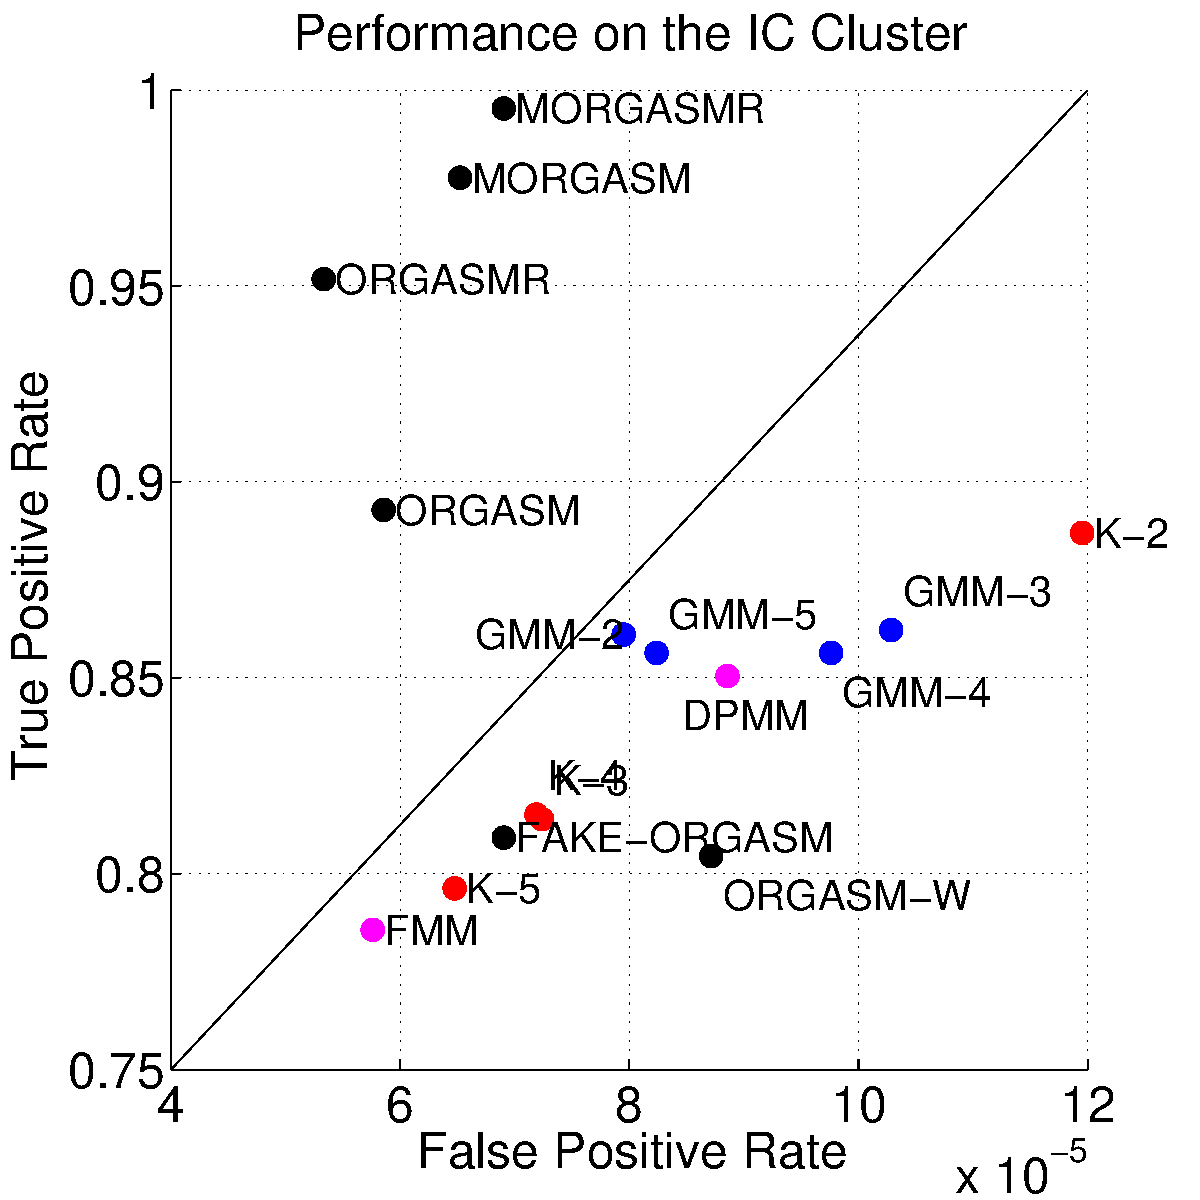
\includegraphics[width=\textwidth]{../figs/truefalsepositive.pdf}
\caption{}
\label{hc1res}
\end{subfigure}
\begin{subfigure}[b]{.49\textwidth}
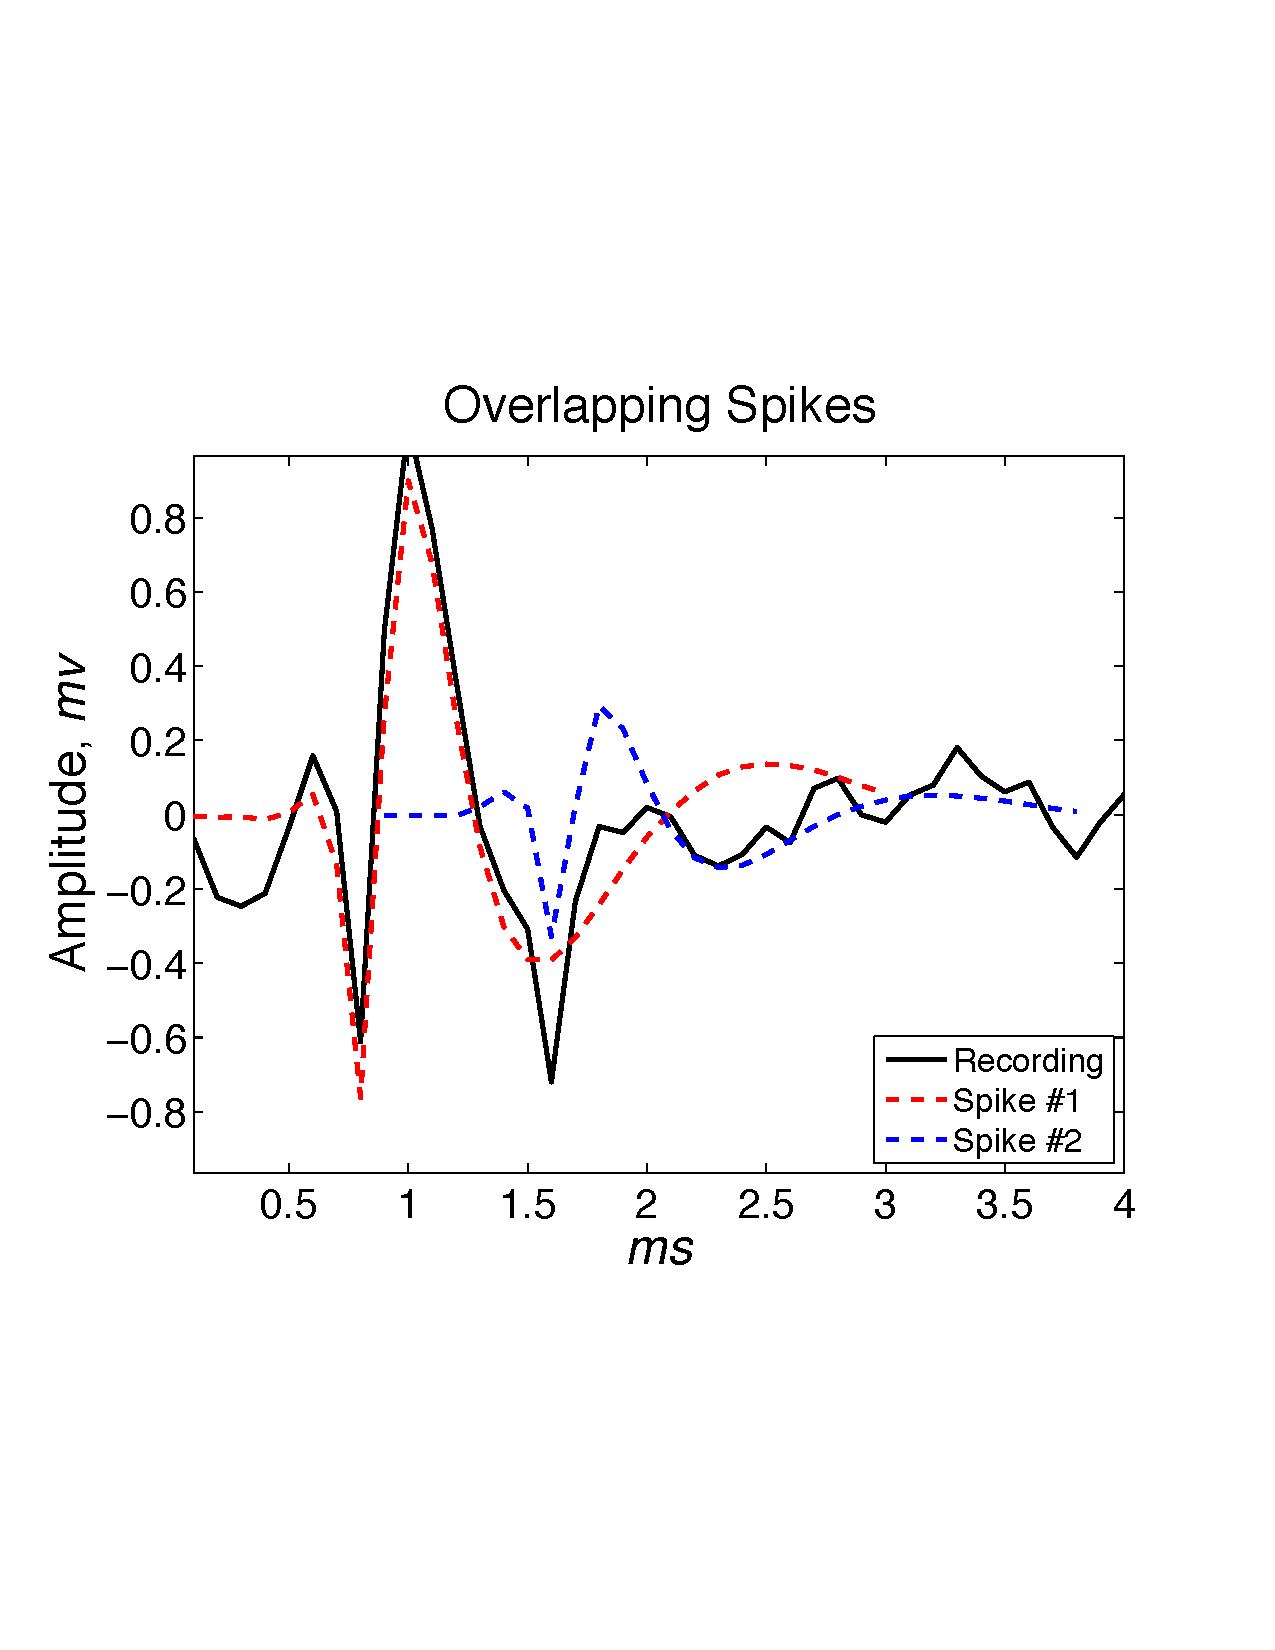
\includegraphics[width=\textwidth]{../figs/alloverlappingspikes/olspike3}
\caption{}
\label{overlapping}
\end{subfigure}



\caption{Results on the d533101 dataset.  (a) This shows the average number of true positives versus the average number of false positives in the intracellular cluster for 2 minute segments of the 4 minutes of day.  The methods that combine the clustering and the detection have similar numbers of false positives but greater numbers of true positives. {\color{red} I have error bars as well, but they look ugly}  (b) An example of an inferred overlapping spike.}
\end{figure}
\end{center}

\subsection{Time-Varying Waveform Adaptation} \label{sub:adapt}
As as been demonstrated previously \cite{calabrese2011kalman}, the waveform shape of a neuron may change over time.  The mean waveform over time for the intracellular neuron is shown in Figure \ref{evohc1}.  Allowing the mean of each component to evolve over time improved single-channel performance over the 4-minute dataset, and gave similar performance in the multi-channel algorithms.
\subsection{Overlapping Spike Detection}
It is possible for action potentials to fire close to simultaneously so that a given window would have 2 or move action potent ions.  It is possible for the algorithm to detect and fit overlapping spikes as they come in.  Out of the 3593 spikes detected by the algorithm, there are 124 pairs of overlapping spikes within 1ms of one another (3.45\%).  An example of an overlapping waveform is shown in Figure \ref{overlapping}.

\subsection{Multi-Electrode Array} \label{sub:multi}

In the tetrode case the waveform undoubtedly appears on all channels at once; it is possible to concatenate the channels to jointly process the data \cite{wood2009}.  When the action potential will only appear on a subset of channels it is nice to allow the action potential to vary in a low-dimensional subset in each of the channels instead of a low-dimensional subset over all the channels. \cite{Prentice2011}

We use processed data from novel NeuroNexus devices implanted in the rat motor cortex.  The data was recorded at 32.5kHz in freely-moving rats, and the data was first processed by high-pass filtering at 800Hz.  The first device we consider is a set of 3 channels of data shown in Figure \ref{3dev}.  The neighboring electrode sites in these devices have 30 $\mu$m between electrode edges and 60 $\mu$m between electrode centers.  These devices are close enough that a locally-firing neuron could appear on multiple electrode sites (cite that paper on action potential overlap), and neighboring channels warrant joint processing.  The second, 8-channel device is shown in Figure \ref{8dev}, and has similar properties to the first device.

 The top 2 clusters found in the first 10 minutes of data on the 3-channel device are shown in Figures \ref{ex31}, \ref{ex32}.  The waveform in channel 3 is very similar for the waveforms in Figure \ref{ex31} and \ref{ex32}, and would be difficult to separate if we were analyzing each channel individually; the representation of those two clusters in PCA space on channel 3 is shown in Figure \ref{chpca}.  We gain the ability to distinguish the waveforms by looking at all the channels simultaneously.  The top 3 clusters found in the 8-channel device can be found in Figures \ref{ex81}, \ref{ex82}, and \ref{ex83}.

{\color{red} perhaps add comments about time-evolution and the false positives we avoid by using multi-channel analysis}

\begin{center}
\begin{figure}
\begin{subfigure}[b]{.5\textwidth}
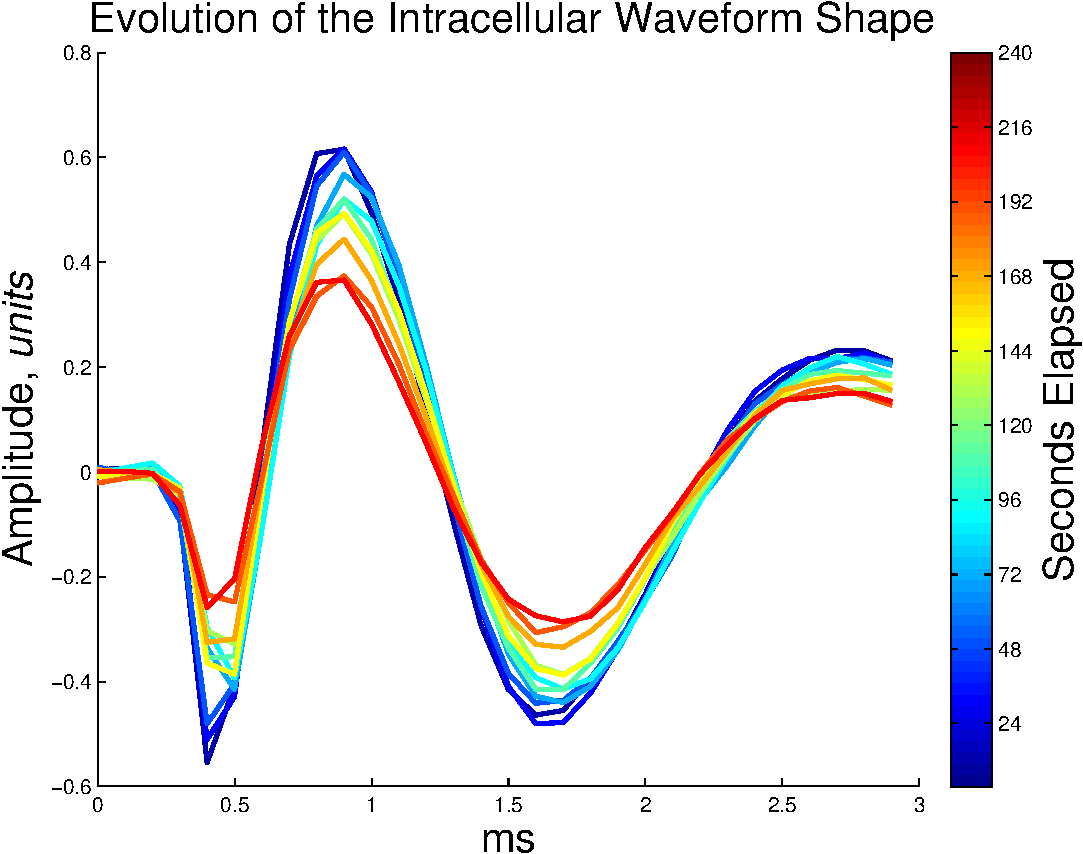
\includegraphics[width=\textwidth]{../figs/evohc1}
\caption{}
\label{evohc1}
\end{subfigure}
\begin{subfigure}[b]{.5\textwidth}
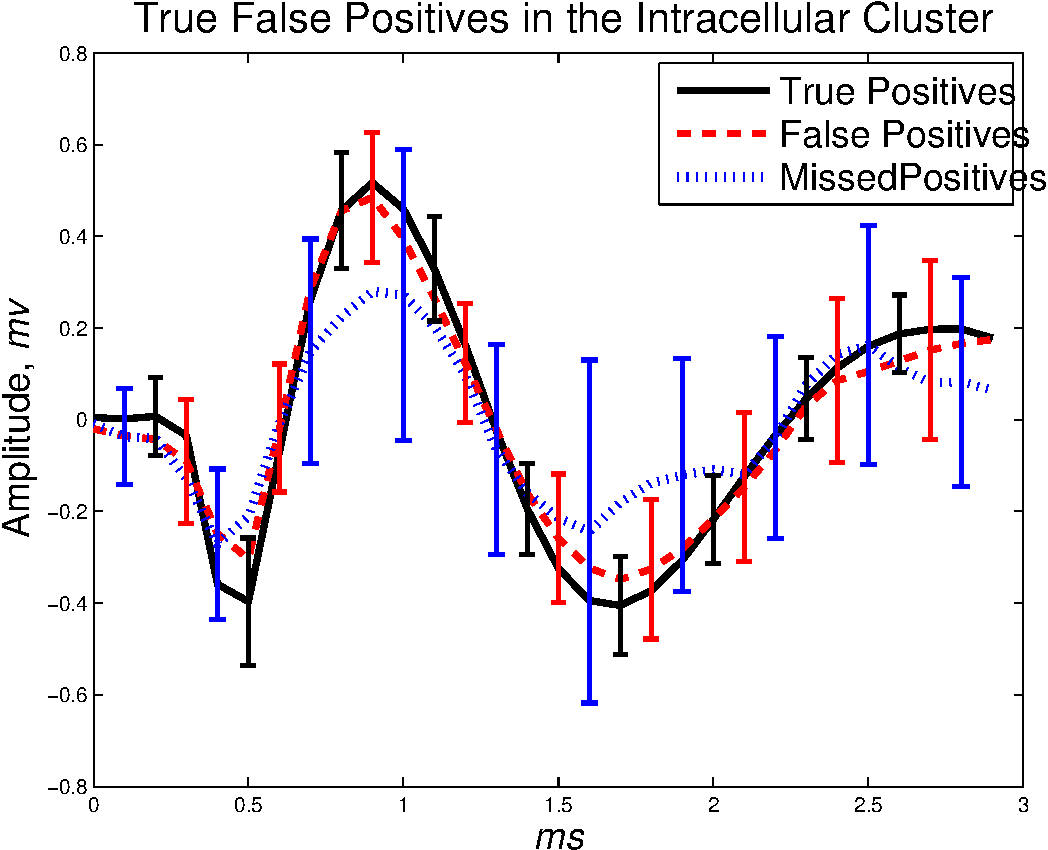
\includegraphics[width=\textwidth]{../figs/IntracellularTrueFalsePositivesv2}
\caption{}
\label{truewaveforms}
\end{subfigure}
\caption{(a) Mean IC waveforms over time.  Each colored line represents the mean of the waveform averaged over 24s and the color gives the elapsed time.  This neuron decreases in amplitude over the period of the recording. (b) Errorbar plots of the true positives and the false positives in the IC cluster.  While the false positives have slightly more variability, the mean shape for the false positives and the true positives is nearly identical.  The true misses have a significantly lower amplitude as well as high variability}
\end{figure}
\end{center}
\begin{center}
\begin{figure}
\begin{subfigure}[b]{.24\textwidth}
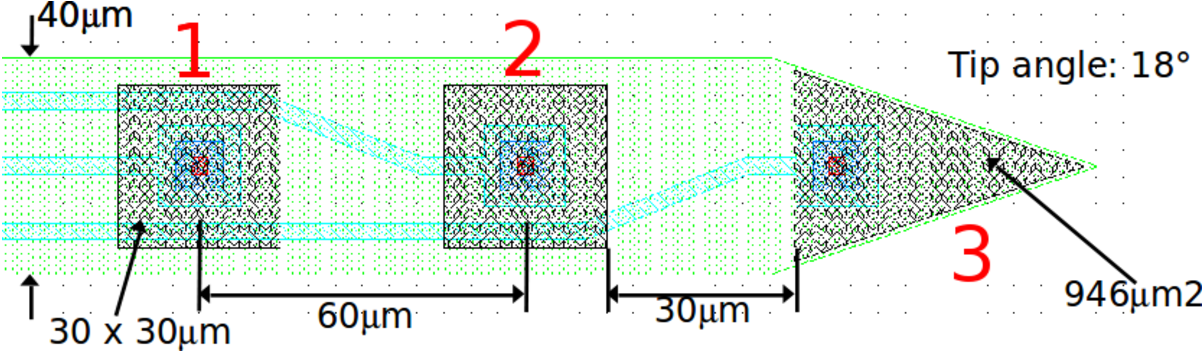
\includegraphics[width=\textwidth]{../figs/3dev}
\caption{}
\label{3dev}
\end{subfigure}
\begin{subfigure}[b]{.24\textwidth}
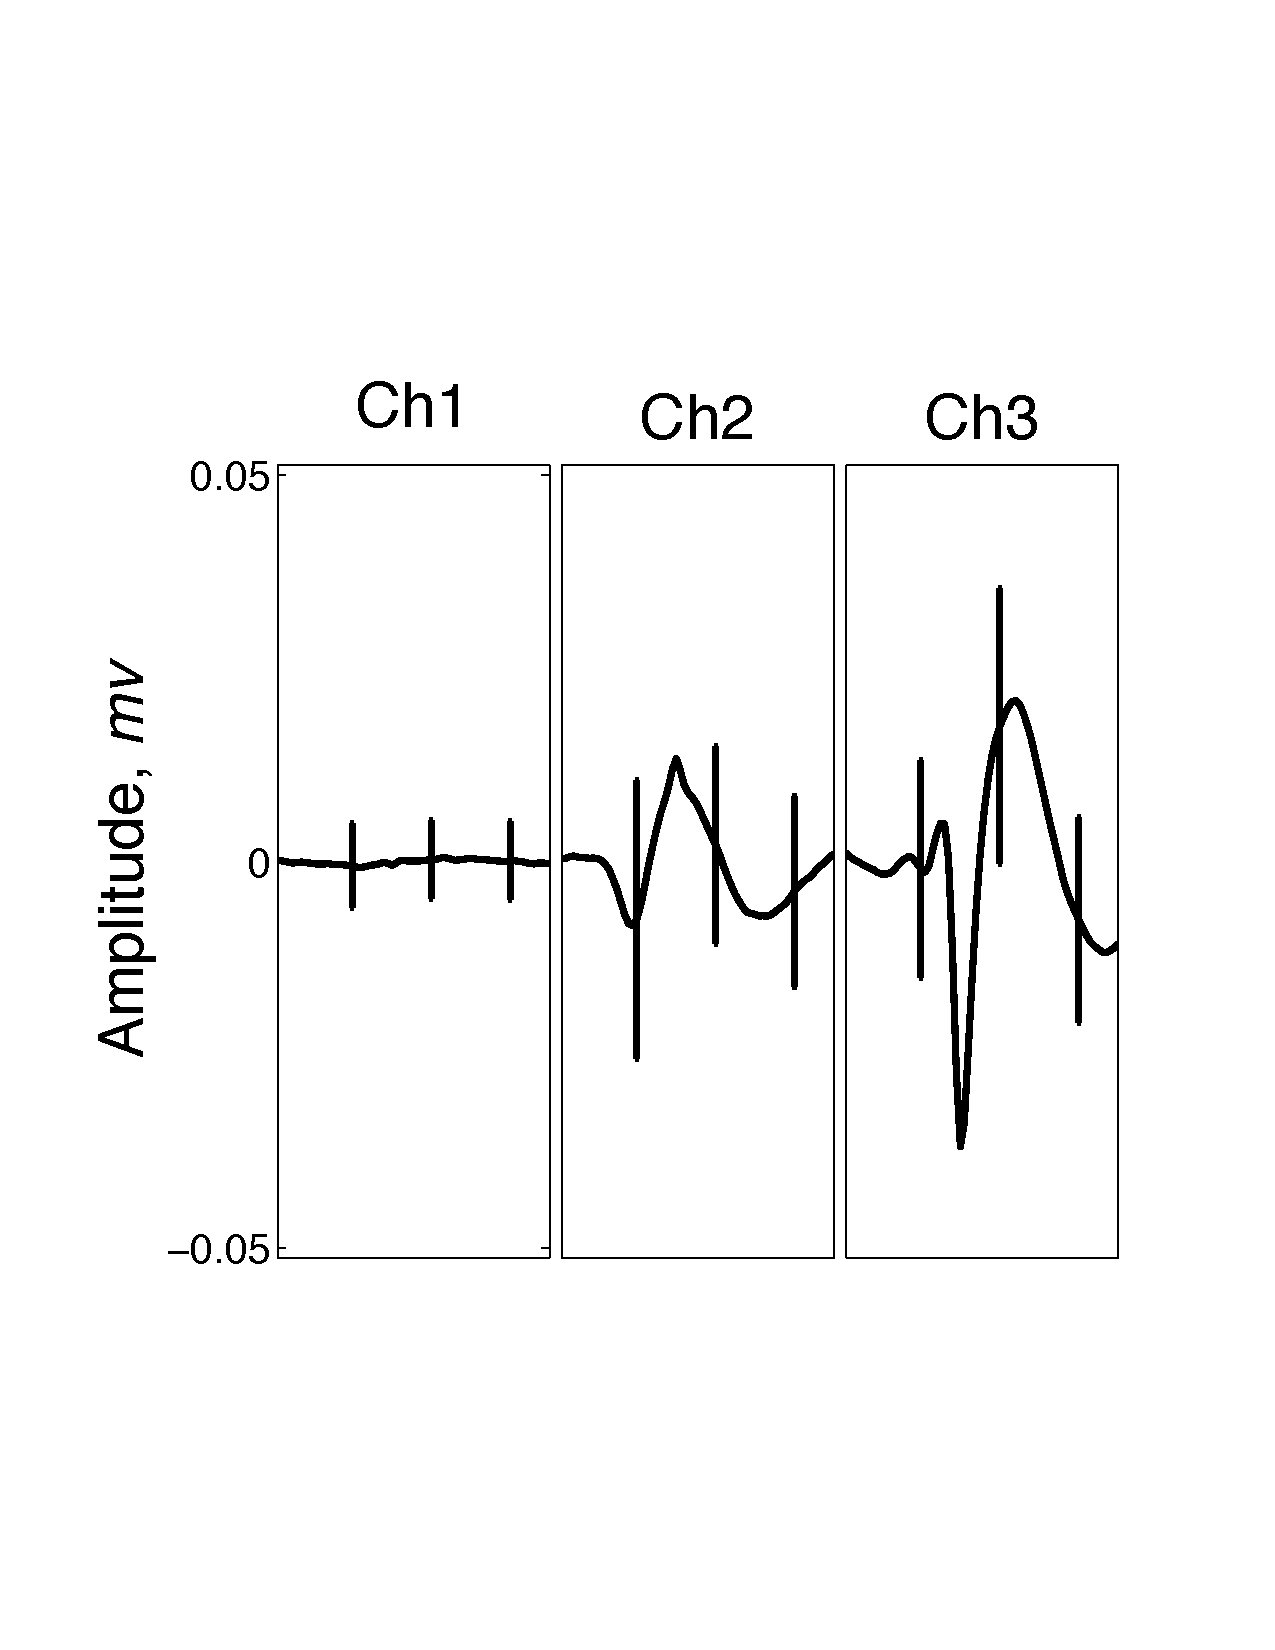
\includegraphics[width=\textwidth]{../figs/3devim/clus1}
\caption{}
\label{ex31}
\end{subfigure}
\begin{subfigure}[b]{.24\textwidth}
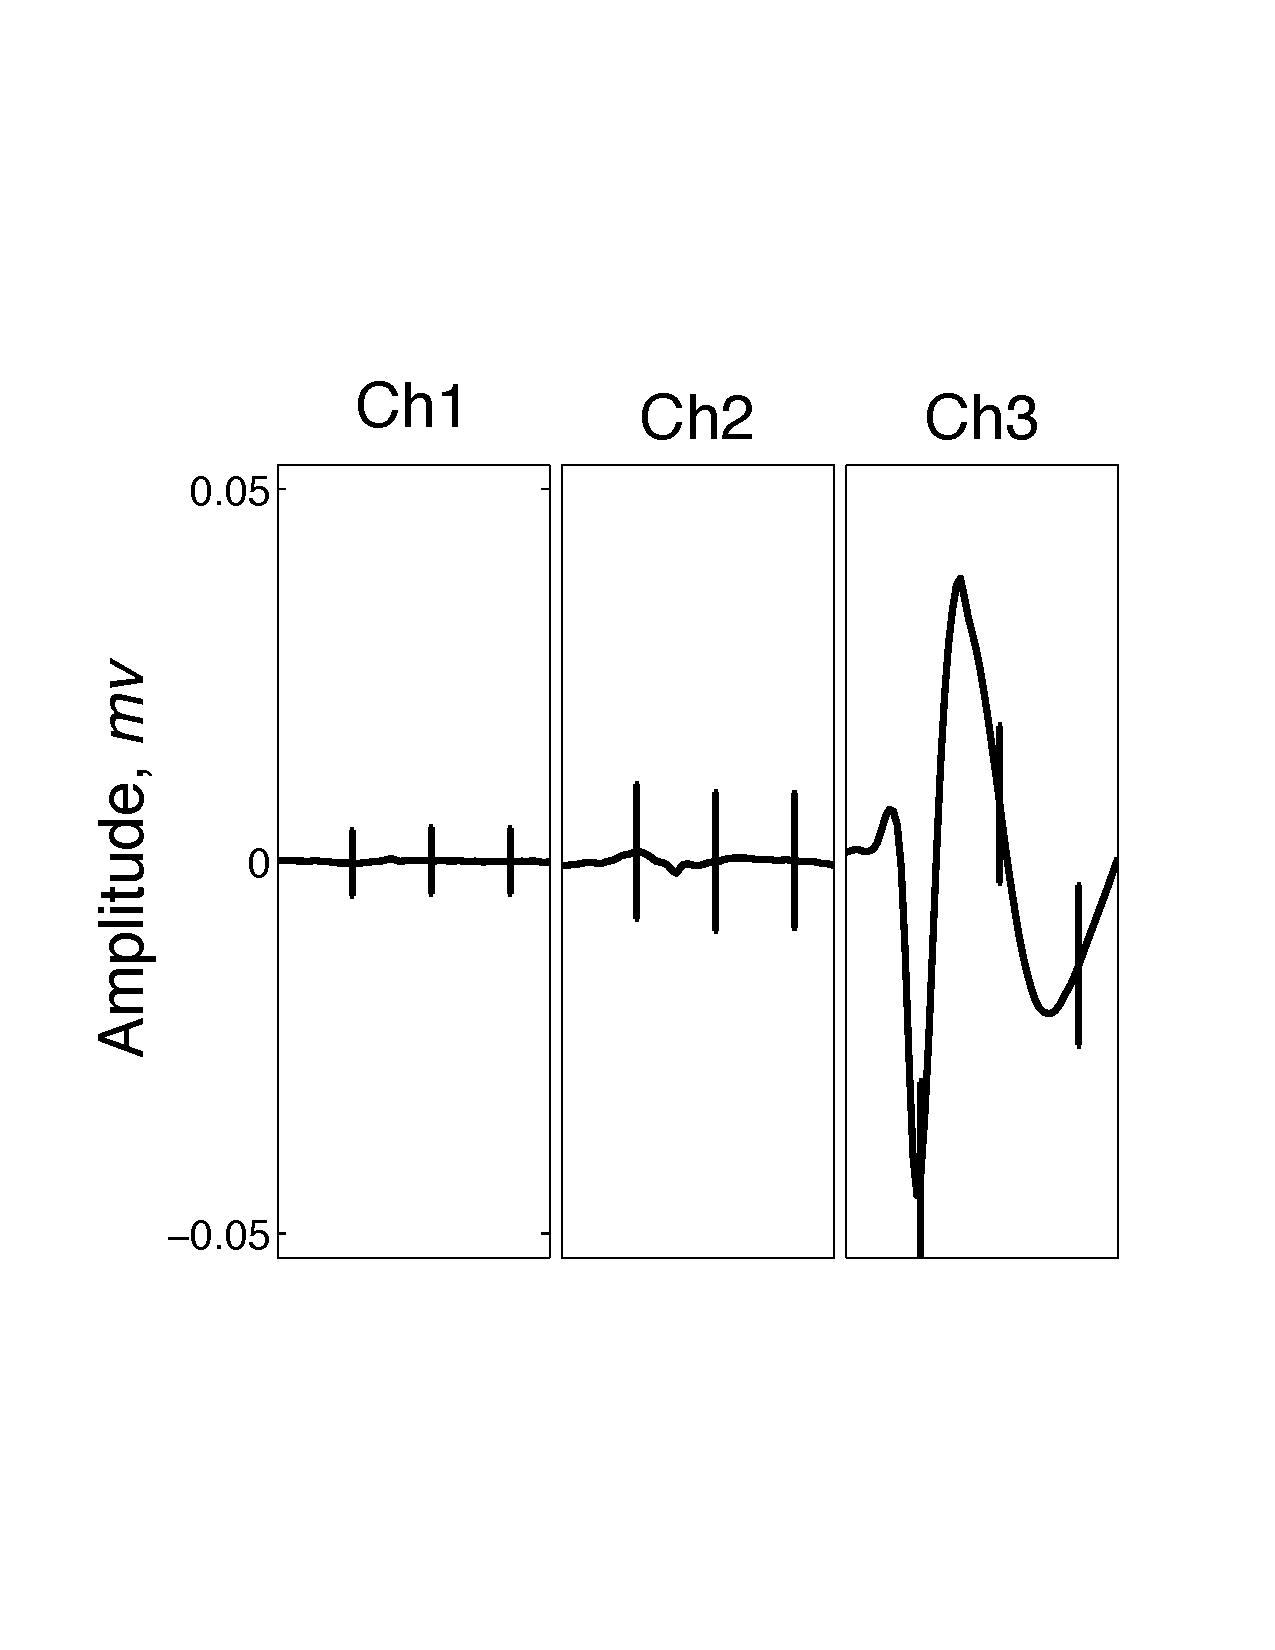
\includegraphics[width=\textwidth]{../figs/3devim/clus2}
\caption{}
\label{ex32}
\end{subfigure}
\begin{subfigure}[b]{.24\textwidth}
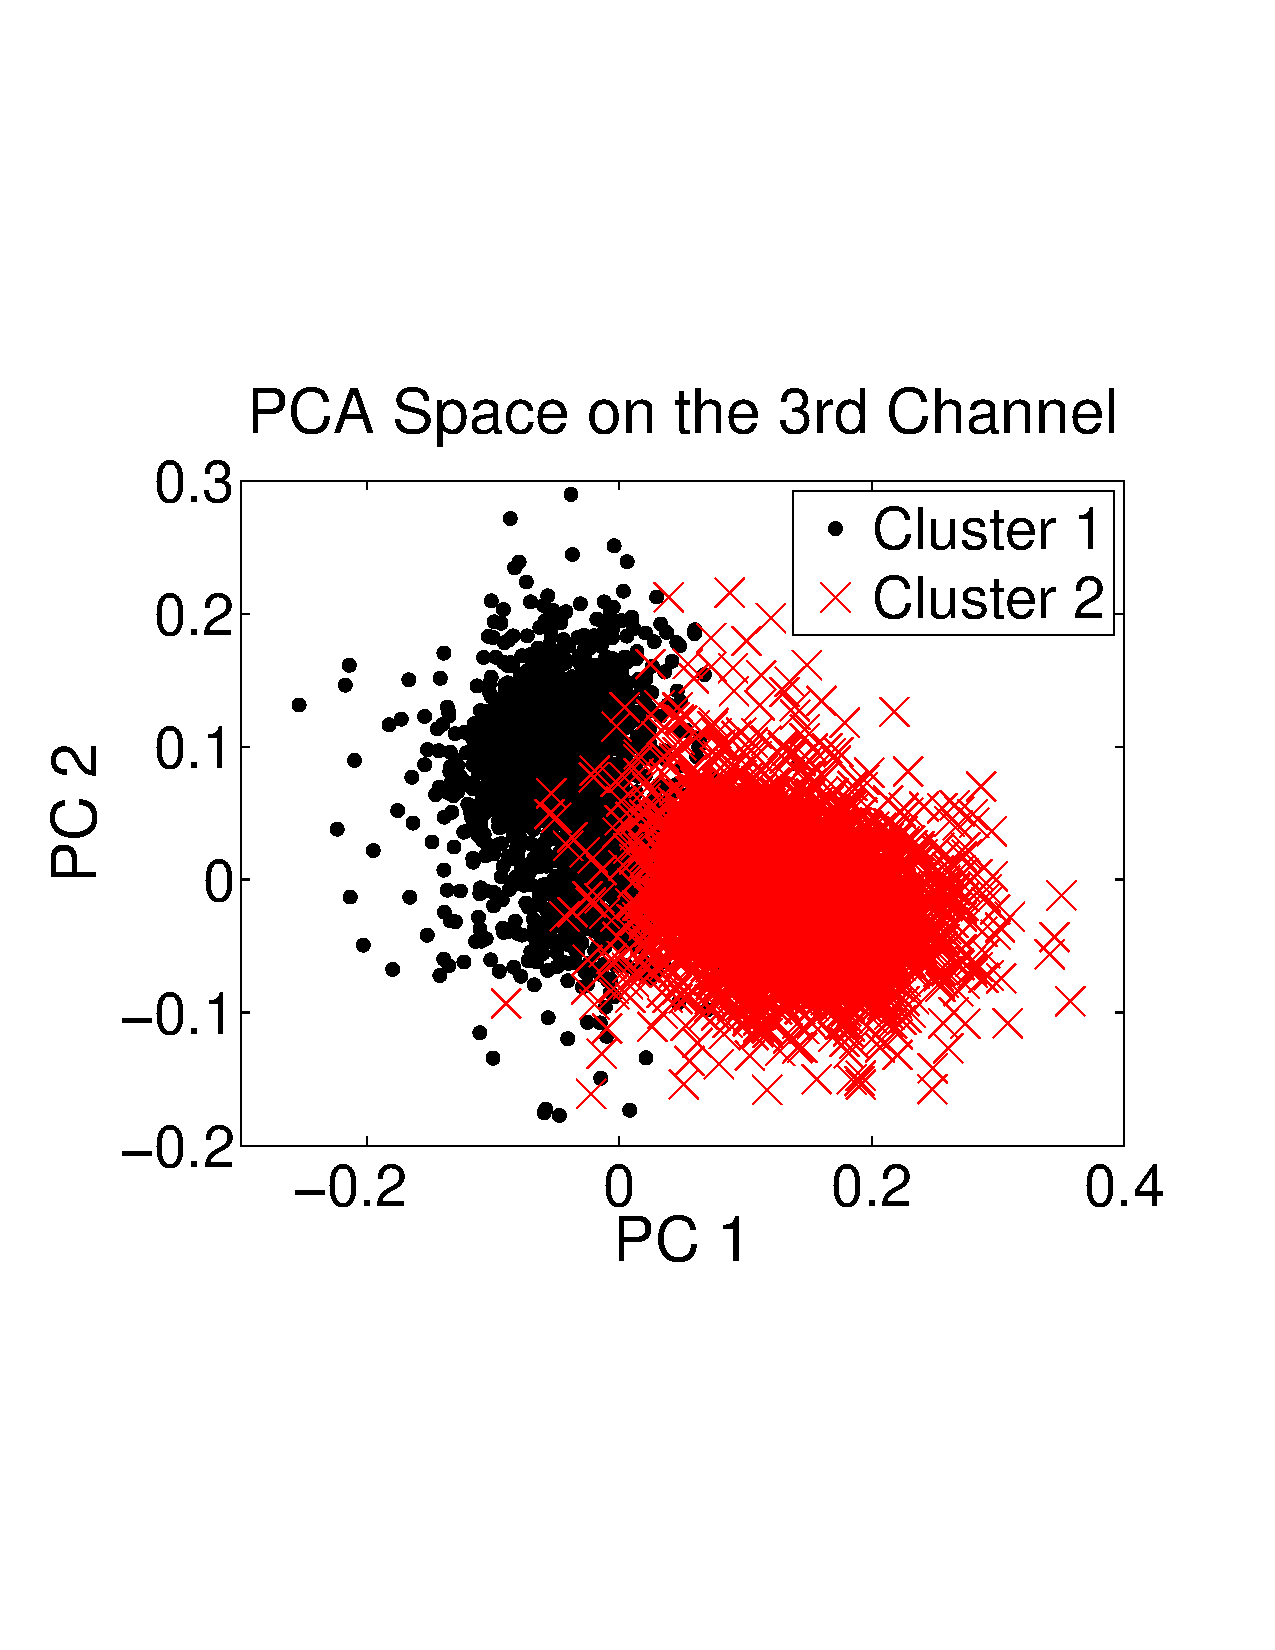
\includegraphics[width=\textwidth]{../figs/new/3chpca}
\caption{}
\label{3chpca}
\end{subfigure}
\caption{(a)3 electrode device showing local proximity of electrodes with channel indexes in large, red numbers. (b,c) Top 2 most prevalent waveforms.  Each waveform shape is 2ms long.   Note in (a) we have a waveform that appears on both channel 2 and channel 3, wheras in (b) the waveform only appears in channel 3.  If only channel 3 was used, it would be difficult to separate the waveform in (a) and (b), as is demonstrated in Figure (d) by the representation of detected spikes on the 3rd channel in PCA space.}
\end{figure}
\end{center}
\begin{center}
\begin{figure}
\begin{subfigure}[b]{.24\textwidth}
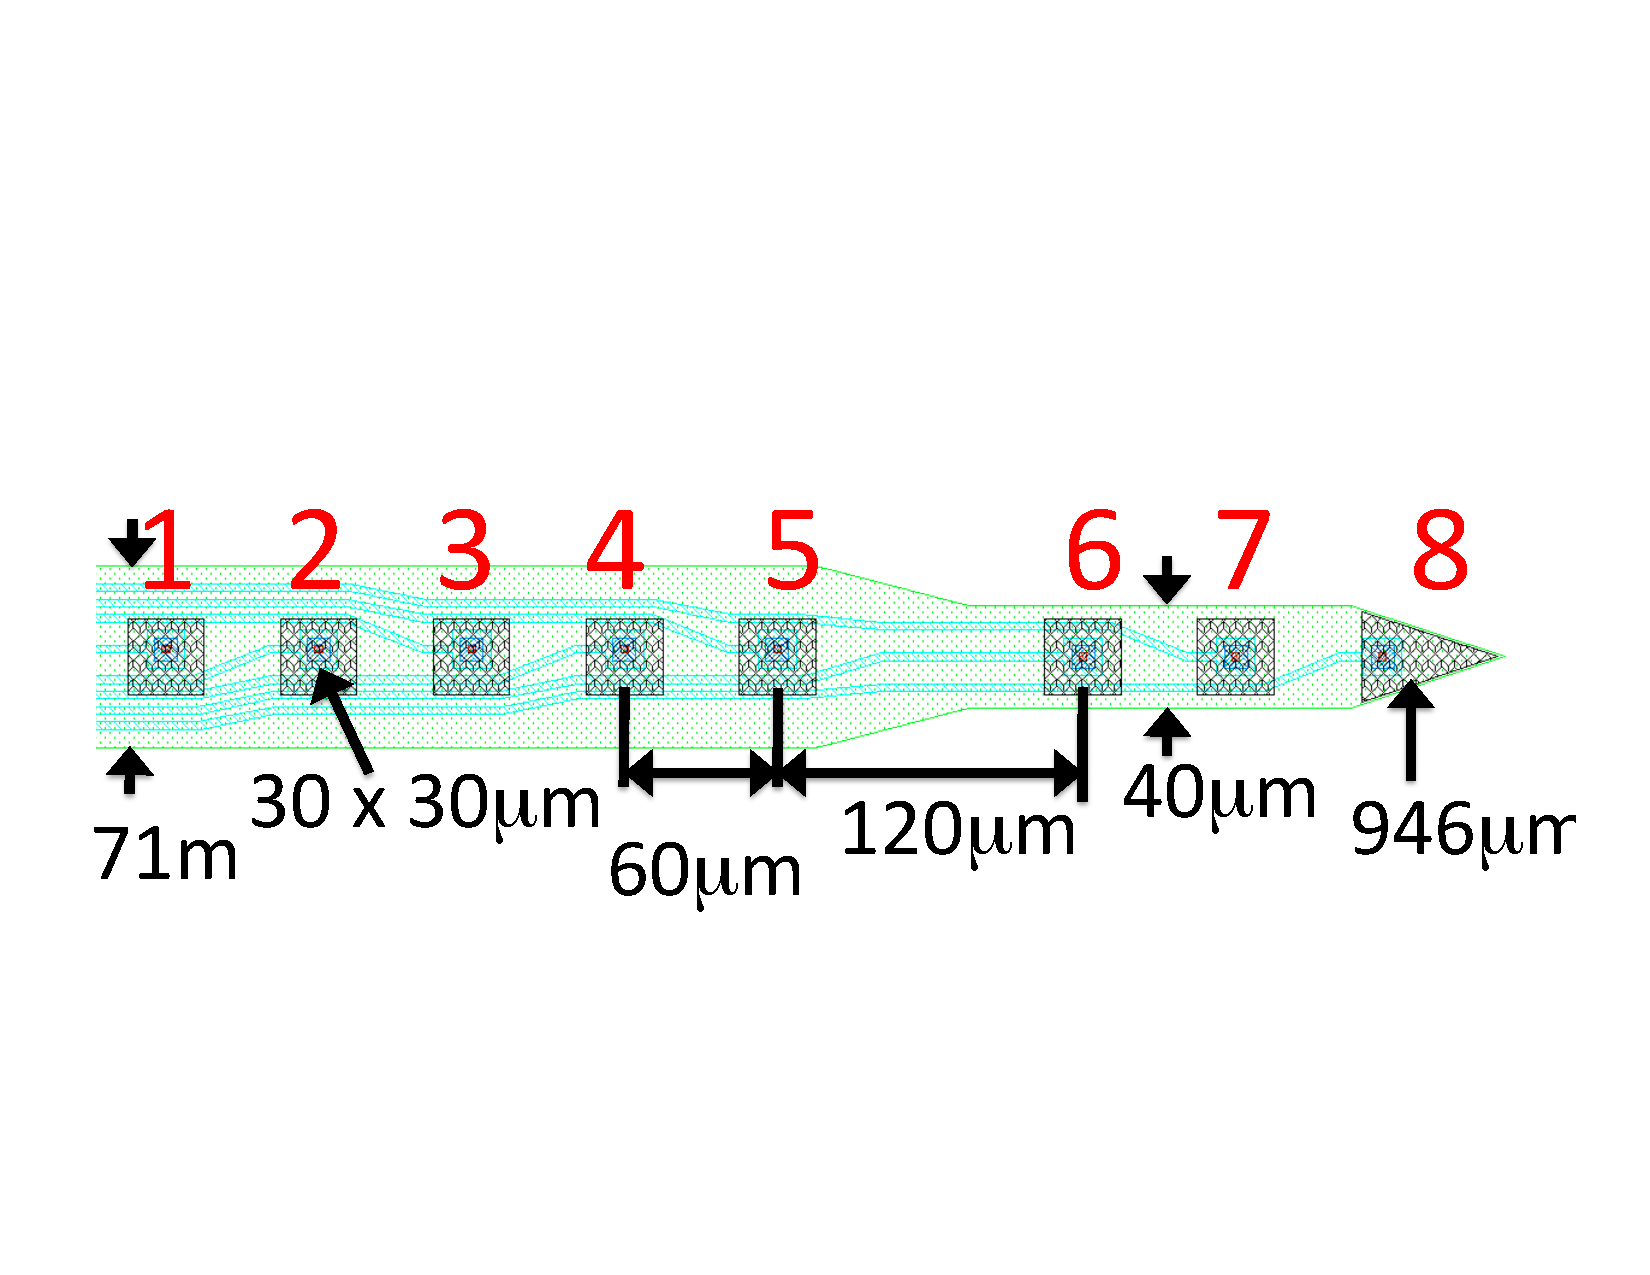
\includegraphics[width=\textwidth]{../figs/8dev}
\caption{}
\label{3dev}
\end{subfigure}
\begin{subfigure}[b]{.24\textwidth}
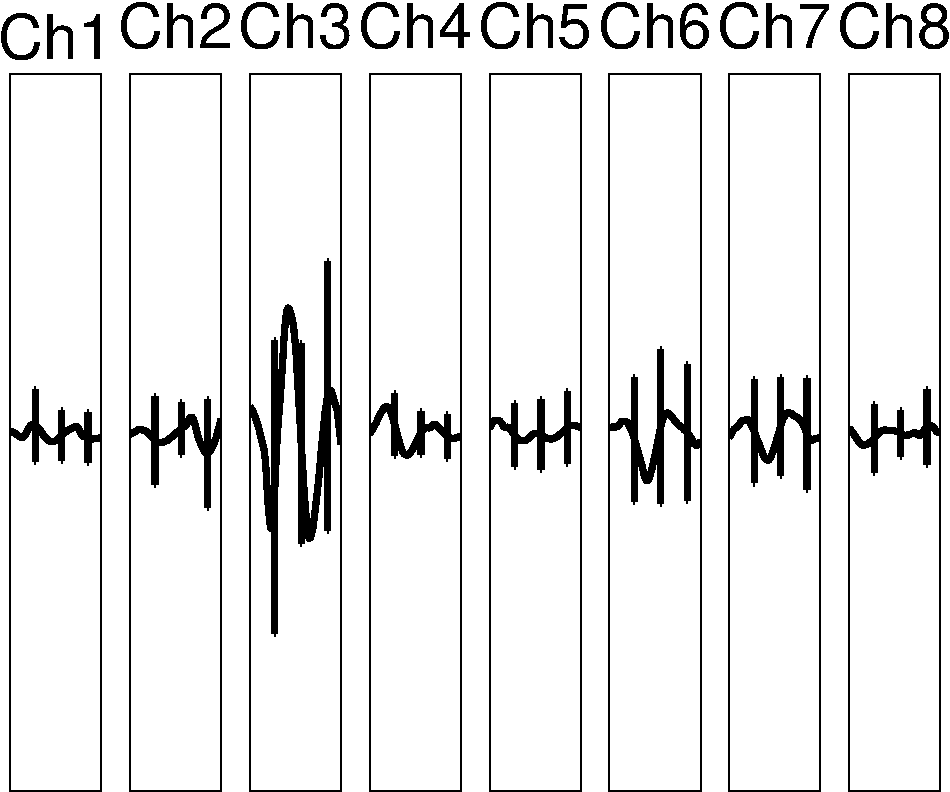
\includegraphics[width=\textwidth]{../figs/8devim/clus3}
\caption{}
\label{ex81}
\end{subfigure}
\begin{subfigure}[b]{.24\textwidth}
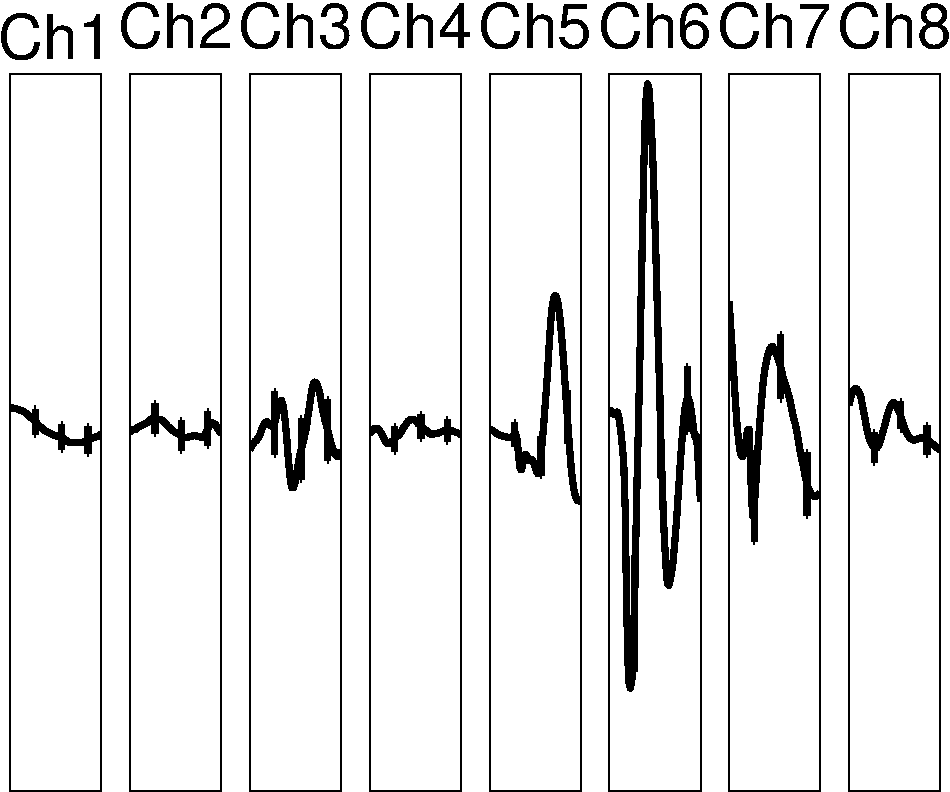
\includegraphics[width=\textwidth]{../figs/8devim/clus9}
\caption{}
\label{ex82}
\end{subfigure}
\begin{subfigure}[b]{.24\textwidth}
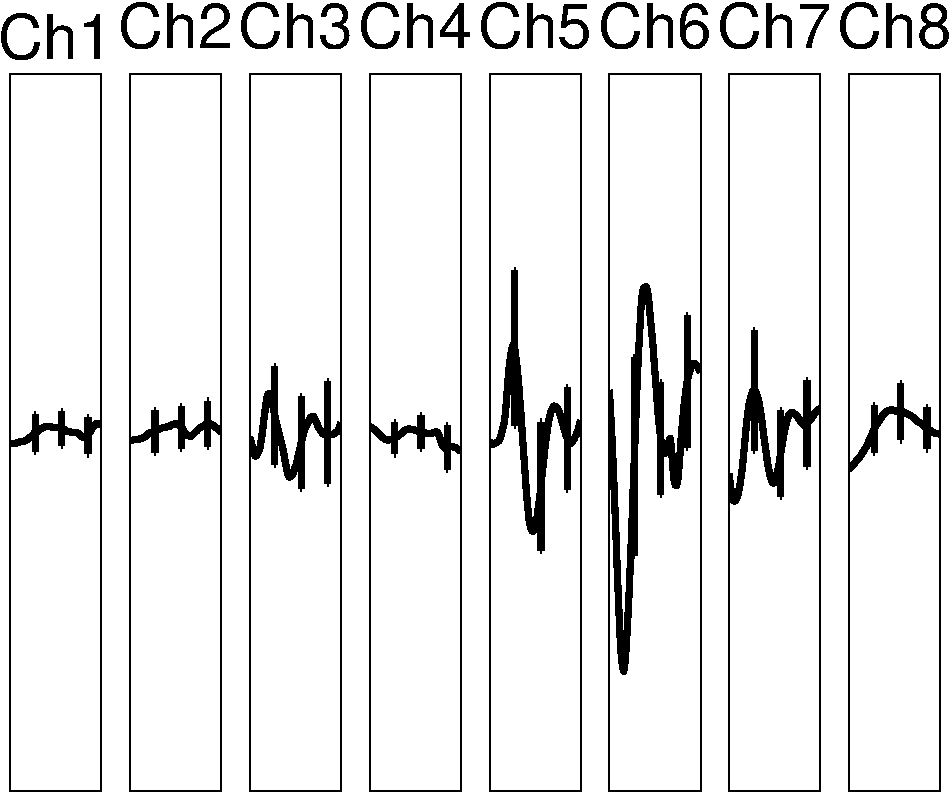
\includegraphics[width=\textwidth]{../figs/8devim/clus6}
\caption{}
\label{ex83}
\end{subfigure}
\caption{(a)8 electrode device showing local proximity of electrodes with channel indexes in large, red numbers. (b,c,d) Top 3 most prevalent waveforms.  Each waveform shape is 2ms long.}
\end{figure}
\end{center}
